%\documentclass[aspectratio=169]{beamer}
\documentclass[handout]{beamer}
%\documentclass{beamer}

% Packages
\usepackage[T1]{fontenc}
\usepackage[utf8]{inputenc}
\usepackage[polish]{babel}
\usepackage[absolute,overlay]{textpos}
%\usepackage[default]{sourcesanspro} % WUT fonts
\usepackage{amsmath, amsthm, amssymb, latexsym}
\usepackage{ragged2e}
\usepackage{lipsum}
\usepackage{tikz}
\usepackage{caption}
\captionsetup[figure]{font=footnotesize,labelfont=footnotesize}
\usepackage{scrbase}
\usepackage{float}
\usepackage{subfig}
\usepackage{lmodern}
\usepackage{listings}

\usetheme{Boadilla}
\makeatother
\setbeamertemplate{headline}{  
  \leavevmode
  \hbox{%
  \begin{beamercolorbox}[wd=.8\paperwidth,ht=2.25ex,dp=1ex,left]{headline}
    \leftskip=10pt \insertsectionhead
  \ifx\insertsubsectionhead\empty\relax\else$\quad\mid\quad$\insertsubsectionhead\fi
  \end{beamercolorbox}%
  \begin{beamercolorbox}[wd=.2\paperwidth,ht=2.25ex,dp=1ex,right]{headline}
    \insertframenumber{} / \inserttotalframenumber\hspace*{1ex}
  \end{beamercolorbox}
  }
  \begin{beamercolorbox}[wd=\paperwidth,ht=0.3cm]{margin}
  \end{beamercolorbox}
}
\setbeamerfont{headline}{size=\scriptsize}
\setbeamertemplate{footline}
{
  \leavevmode
  \begin{beamercolorbox}[wd=\paperwidth,ht=0cm]{margin}
  \end{beamercolorbox}

 
  \begin{beamercolorbox}[wd=\paperwidth,ht=.5cm]{footline}
    \begin{columns}
   	\begin{column}{1.0\paperwidth}
   	\href{https://github.com/egi-megi/rojCzastek_Szczepanski_Jurkiewicz_Pikulinski}{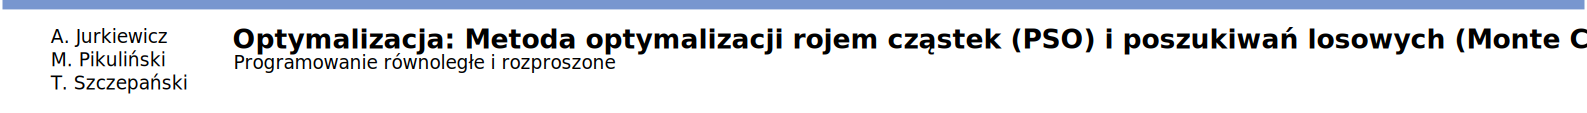
\includegraphics[width=1.0\paperwidth,keepaspectratio]{grafiki/footer}}

   	\end{column}
    \end{columns}
  \end{beamercolorbox}
}
\makeatletter
\setbeamertemplate{navigation symbols}{}
\setbeamersize{text margin left=8mm,text margin right=8mm} 

%Defined colors
\definecolor{mainColor}{RGB}{120,150,207}
\definecolor{lightgray}{RGB}{180,160,170}
\definecolor{additional}{RGB}{60,60,76}

\setbeamercolor{headline}{fg=white,bg=mainColor}
\setbeamercolor{footline}{fg=black, bg=white}

\setbeamercolor{normal text}{fg=black, bg=white}
\setbeamercolor{block title}{fg=white,bg=mainColor}
\setbeamercolor{block body}{fg=black,bg=lightgray}
%\setbeamertemplate{blocks}[rounded][shadow=true]

\setbeamertemplate{itemize items}[circle]
\setbeamercolor{enumerate item}{fg=mainColor,bg=white}
\setbeamercolor{enumerate subitem}{fg=mainColor,bg=white}
\setbeamercolor{enumerate subsubitem}{fg=mainColor,bg=white}

\setbeamercolor{itemize item}{fg=mainColor,bg=white}
\setbeamercolor{itemize subitem}{fg=mainColor,bg=white}
\setbeamercolor{itemize subsubitem}{fg=mainColor,bg=white}

\definecolor{mycolor1}{RGB}{0,0,128}
\definecolor{lightgray}{gray}{0.9}
\definecolor{lightlightgray}{gray}{0.95}
\definecolor{lightyellow}{RGB}{255,255,224}
\definecolor{lemonchiffon}{RGB}{255,250,205}
\definecolor{syntax}{RGB}{127,0,85}
\definecolor{comments}{RGB}{63,127,95}
\definecolor{strings}{RGB}{42,0,255}

\lstdefinestyle{mycpp} {
    language=C, % choose the language of the code
    alsolanguage=C++,
    basicstyle=\linespread{0.9}\fontfamily{lmtt}\selectfont\small\color{black},
    keywordstyle={\bfseries\color{syntax}}, % style for keywords
    emph={int,char,double,float,unsigned,printf,getchar,putchar,
sprintf,scanf,fopen,fscanf,fprintf,fclose,pthread_self,pthread_create,sleep,exit,pthread_t,
pthread_exit,pthread_cancel,pthread_join,pthread_attr_init,pthread_attr_setdetachstate,pthread_attr_destroy,
pthread_attr_getdetachstate,pthread_attr_setdetachstate,pthread_attr_getinheritsched,pthread_attr_setinheritsched,
pthread_attr_getschedpolicy,pthread_attr_setschedpolicy,pthread_attr_getschedparam,pthread_attr_setschedparam,
pthread_attr_getscope,pthread_attr_setscope,pthread_attr_getstacksize,pthread_attr_getstackaddr,pthread_attr_setstacksize,
pthread_attr_setstackaddr,pthread_attr_t,srand,time,rand,pthread_mutex_init,pthread_mutex_t,pthread_mutex_destroy,
pthread_mutex_lock,pthread_mutex_timedlock,time_t,pthread_mutex_trylock,pthread_mutex_unlock,
pthread_cond_init,pthread_cond_destroy,pthread_cond_wait,pthread_cond_timedwait,pthread_cond_signal,pthread_cond_broadcast,
pthread_barrier_init, pthread_barrier_t,pthread_barrierattr_t,pthread_barrier_wait,pthread_barrier_destroy,
pthread_cond_t,pthread_mutexattr_t,pthread_condattr_t,ChannelCreate,ChannelCreate_r,
ChannelDestroy,ChannelDestroy_r,ChannelAttach,ChannelDetach,MsgReceive,MsgReply,MsgSend,strerror,ConnectAttach,ConnectAttach_r,
pid_t,uint32_t,ConnectDetach,ConnectDetach_r,MsgSend_r,MsgReceive_r,name_attach,name_detach,name_open,name_close,
open,MsgReply_r,atoi,strcpy,_uint16,_int8,_uint8,_int32,MsgSendPulse,MsgReceivePulse,clock_gettime,perror,
clock_getres,clock_settime,ctime,nanosleep,delay,select,alarm,nanospin,timer_create,timer_settime,timer_gettime,timer_delete,
getpid},
    emphstyle={\bfseries\color{syntax}},
    stringstyle=\color{strings},
    commentstyle={\fontfamily{lmtt}\selectfont\color{comments}},
    numbers=left, % where to put the line-numbers
    numberstyle=\tiny, % the size of the fonts that are used for the line-numbers
    %backgroundcolor=\color{lemonchiffon},
    backgroundcolor=\color{lightgray},
    showspaces=false, % show spaces adding particular underscores
    showstringspaces=false, % underline spaces within strings
    showtabs=false, % show tabs within strings adding particular underscores
    frame=single, % adds a frame around the code
    tabsize=2, % sets default tabsize to 2 spaces
    rulesepcolor=\color{gray},
    rulecolor=\color{black},
    captionpos=t, % sets the caption-position to bottom
    breaklines=true, % sets automatic line breaking
    breakatwhitespace=false,
    xleftmargin=20pt,
    xrightmargin=20pt,
    aboveskip=12pt,
    belowskip=12pt,
    escapeinside={(*@}{@*)},
%   frameround=tttt,
   framexleftmargin=5mm,
   frame=shadowbox,
   rulesepcolor=\color{lightgray},
   extendedchars=\true,
   inputencoding=utf8,
}

\renewcommand*\lstlistingname{Kod źródłowy}

% font sizes
\renewcommand*{\tiny}{\fontsize{4}{5}\selectfont}
\renewcommand*{\scriptsize}{\fontsize{6}{7.2}\selectfont}
\renewcommand*{\footnotesize}{\fontsize{8}{9.6}\selectfont}
\renewcommand*{\small}{\fontsize{8}{9.6}\selectfont}
\renewcommand*{\normalsize}{\fontsize{10}{12}\selectfont}
\renewcommand*{\large}{\fontsize{11}{13.3}\selectfont}
\renewcommand*{\Large}{\fontsize{12}{14.4}\selectfont}
\renewcommand*{\LARGE}{\fontsize{14}{16.8}\selectfont}
\renewcommand*{\huge}{\fontsize{17}{20.4}\selectfont}
\renewcommand*{\Huge}{\fontsize{20}{34}\selectfont}

\date{19.01.2021}
\title{Optymalizajca: Metoda optymalizacji rojem cząstek (PSO) i poszukiwań losowych (Monte Carlo)}
\institute{Politechnika Warszawska}

\usepackage{mathtools}
\usepackage{cases}
\usepackage{siunitx}

\apptocmd{\frame}{}{\justifying}{}

\usepackage{bm}
\newcommand{\matr}[1]{\mathbf{#1}}
\newcommand{\vect}[1]{\bm{\mathbf{#1}}}
\newcommand{\integrand}[1]{\left(#1\right)}
\DeclareRobustCommand*{\drv}{\mathop{}\!\mathrm{d}}
\DeclareRobustCommand*{\intdt}{\mathop{}\!\mathrm{dt}}


%\renewcommand{\raggedright}{\justifying}
\usefonttheme{professionalfonts} % Naprawia problem z capital greek Phi
\addtobeamertemplate{frametitle}{\vskip-0.8ex}{}
\setbeamercolor{frametitle}{fg=black}

\usepackage{animate}
\usepackage{caption}
\captionsetup[figure]{font=scriptsize,labelfont=scriptsize}
\setbeamerfont{caption}{size=\tiny}

\setlength{\belowdisplayskip}{0pt}
\newcommand{\lenitem}[2][.4\linewidth]{\parbox[t]{#1}{\strut #2\strut}}

\begin{document}


\begin{frame}


\begin{center}
\vspace{.3cm}
Optymalizacja \\

\vspace{.3cm}
{\LARGE \textbf{Metoda optymalizacji rojem cząstek (PSO) \\ i poszukiwań losowych (Monte Carlo)}}

\vspace{.8cm}
{\Large Doświadczenia z implementacji C++} \\
\vspace{.2cm}
{\Large OpenMP, MPI, CUDA} \\

\vspace{1.2cm}
{\small Programowanie równoległe i rozproszone \\ sem. zimowy 2020/2021}
\end{center}


\end{frame}




\section{Wstęp teoretyczny}
\subsection{Rój cząstek (PSO)}
\begin{frame}{Rój cząstek (PSO)}

\vspace{-.7cm}
\begin{columns}
\begin{column}[t]{0.5\textwidth}

\begin{figure}[t]
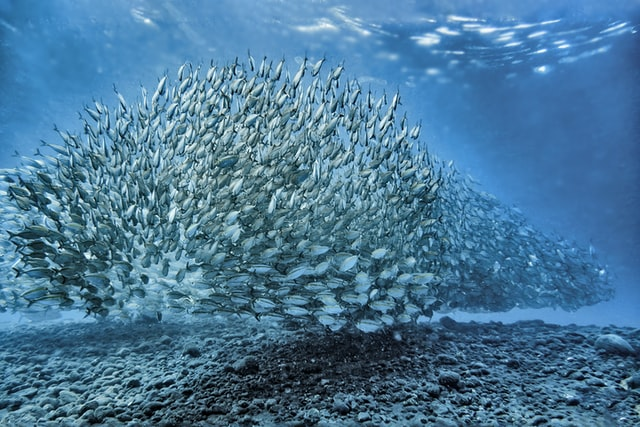
\includegraphics[width=0.9\textwidth]{grafiki/lawicaRyb.jpg}
\captionof{figure}{Ławica ryb (Photo by Dorothea OLDANI on Unsplash)}
\end{figure}

\end{column}
\begin{column}[t]{0.5\textwidth}

\begin{figure}[t]
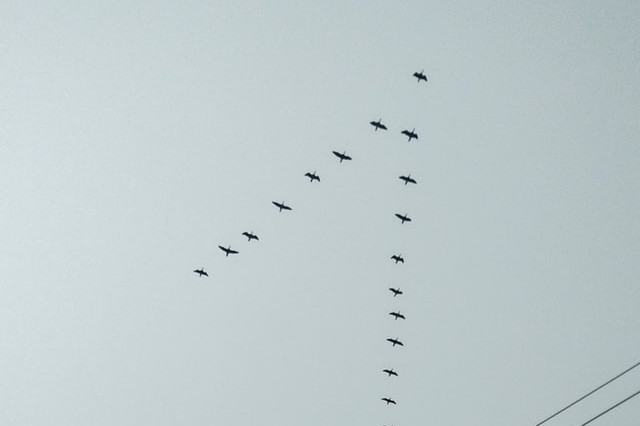
\includegraphics[width=0.9\textwidth]{grafiki/kluczPtakow.jpg}
\captionof{figure}{Klucz ptaków (Photo by Inu Etc on Unsplash)}
\end{figure}

\end{column}
\end{columns}

Matematycznie, zachowanie $j$-tej cząstki w $k$-elementowej populacji:
\begin{equation}
\begin{cases}
\vect{v}_{i + 1, j} = \omega \vect{v}_{i, j} + c_{1} \epsilon_{1} \left(\vect{p}_{i, j} - \vect{x}_{i, j}\right) + c_{2} \epsilon_{2} \left(\vect{q}_{i} - \vect{x}_{i, j}\right) \\
\vect{x}_{i + 1, j} = \vect{x}_{i, j} + \vect{v}_{i + 1, j},
\end{cases}
\end{equation}
gdzie $\vect{x}_{i, j}$ i $\vect{v}_{i, j}$ to odpowiednio wektory położenia i prędkości w generacji $i$, zmienne skalarne $\omega$, $c_1$, $c_2$ to wagi, a $\epsilon_{1}$ i  $\epsilon_{2}$ to pewne zmienne losowe.


\end{frame}

\subsection{Monte Carlo}
\begin{frame}{Monte Carlo}
Położenia cząstki w kolejnych generacjach w tym algorytmie można opisać zgodnie z następującym schematem
\begin{equation}
\vect{\overline{x}}_{i + 1, j} = \vect{x}_{i, j} + \sigma\vect{\xi},
\end{equation}
gdzie $\sigma$ to waga, a $\vect{\xi}$ to $n$-wymiarowa zmienna o rozkładzie jednostajnym. Zmienna $\vect{\overline{x}}_{i + 1, j}$ zostanie zaakceptowana jako nowa współrzędna cząstki $\vect{x}_{i + 1, j} = \vect{\overline{x}}_{i + 1, j}$, jeżeli funkcja celu $f\left(\vect{\overline{x}}_{i + 1, j}\right) < f\left(\vect{x}_{i, j}\right)$. W przeciwnym wypadku rozpatrywane są dwie możliwości.

Dodatkowo losowana jest zmienna $z$ o jednostajnym rozkładzie na przedziale $\left[0, \ 1 \right]$. Jeżeli spełniony będzie warunek
\begin{equation} \label{eq:mc_nie}
z < e^{-\frac{f\left(\vect{\overline{x}}_{i + 1, j}\right) - f\left(\vect{x}_{i, j}\right)}{T}},
\end{equation}
to nowe położenie, pomimo większej wartości funkcji celu, zostanie zaakceptowane ($T$ to parametr). Jeżeli nierówność (\ref{eq:mc_nie}) nie będzie spełniona, to cząstka w danej generacji nie zmieni swojego położenia $\vect{x}_{i + 1, j} = \vect{x}_{i, j}$. 
\end{frame}




\subsection{Zadania optymalizacji}
\begin{frame}{Zadania optymalizacji}

\vspace{-.7cm}
\begin{columns}
\begin{column}[t]{0.5\textwidth}

\begin{tiny}
\begin{equation}
\min_{x} \left(f_{1}\left(\vect{x}\right) = \frac{1}{40} \sum_{i=1}^{n}\left(x_{i}\right)^{2} + 1 - \prod_{i =1}^{n} \cos\left(\frac{x_{i}}{i}\right)\right)
\end{equation}
\begin{equation}
-40 \leq x_{i} \leq 40 \quad i = 1, \ ..., \ n,
\end{equation}
\end{tiny}


\vspace{-.3cm}

\begin{figure}[t]
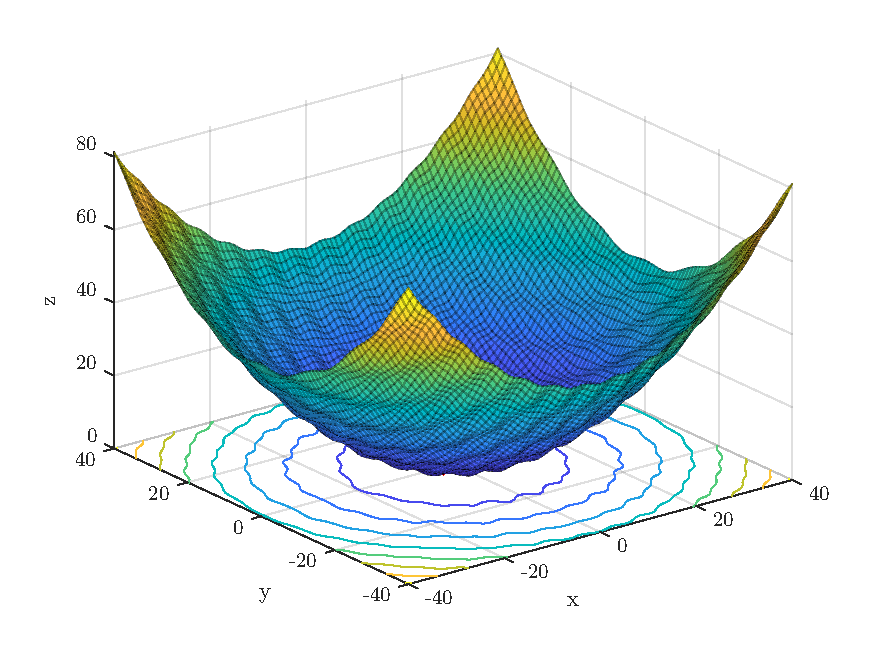
\includegraphics[width=0.9\textwidth]{grafiki/zad_1.pdf}
\captionof{figure}{Zadania 1. (pełna dziedzina).}
\end{figure}

\end{column}
\begin{column}[t]{0.5\textwidth}

\begin{tiny}
\begin{equation}
\min_{x} \left(f_{2}\left(\vect{x}\right) = \sum_{i=1}^{n-1}\left(100\left(x_{i+1}-x_{i}^{2}\right)^{2} + \left(1-x_{i}\right)^{2} \right) \right)
\end{equation}
\begin{equation}
-40 \leq x_{i} \leq 40 \quad i = 1, \ ..., \ n,
\end{equation}
\end{tiny}

\vspace{-.3cm}

\begin{figure}[t]
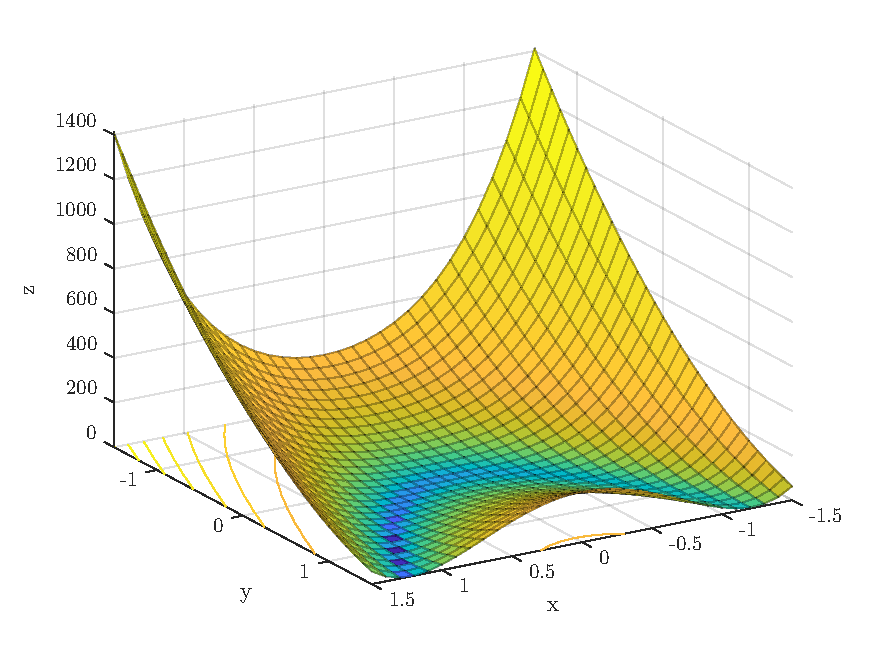
\includegraphics[width=0.9\textwidth]{grafiki/zad_2.pdf}
\captionof{figure}{Zadanie 2. (ograniczona dziedzina).}
\end{figure}

\end{column}
\end{columns}
\end{frame}




\section{Implementacje}
\subsection{Sekwencyjnie}

\begin{frame}{Algorytm sekwencyjnie}
\begin{figure}[t]
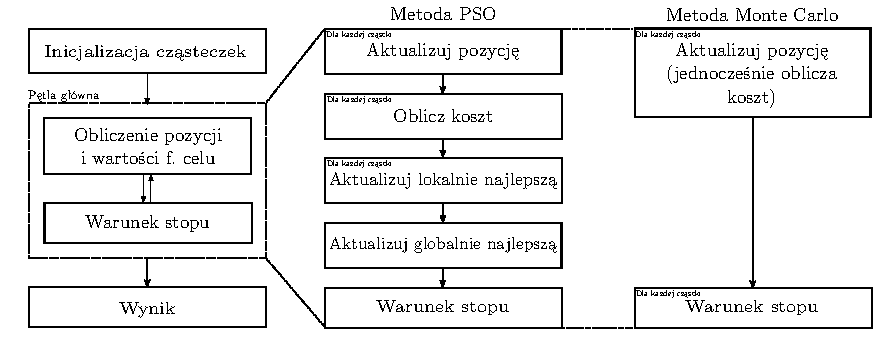
\includegraphics[width=1\textwidth]{grafiki/alg_szczegolowy.pdf}
\end{figure}
\end{frame}

\subsection{MPI}

\begin{frame}{Implementacja PSO w MPI}
\begin{figure}[t]
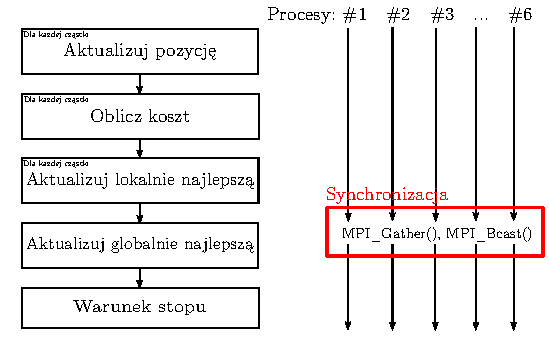
\includegraphics[width=0.9\textwidth]{grafiki/alg_MPI_PSO.pdf}
\end{figure}
\end{frame}

\begin{frame}{Implementacja Monte Carlo w MPI}
\begin{figure}[t]
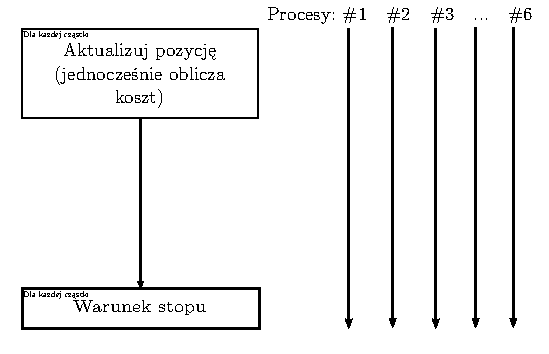
\includegraphics[width=0.9\textwidth]{grafiki/alg_MPI_MC.pdf}
\end{figure}
\end{frame}

\begin{frame}{Podsumowanie MPI}
\begin{itemize}
\item Przyspieszenie dla PSO jest znacznie mniejsze niż  dla Monte Carlo.
\item Nie zawsze w każdym z procesów jest wykonana taka sama liczba iteracji -- procesy te nie startują jednocześnie, ponieważ mają opóźnienia spowodowane koniecznością komunikacji.
\end{itemize}
\vspace{-.3cm}
\begin{columns}
\begin{column}[t]{0.5\textwidth}

\begin{figure}[t]
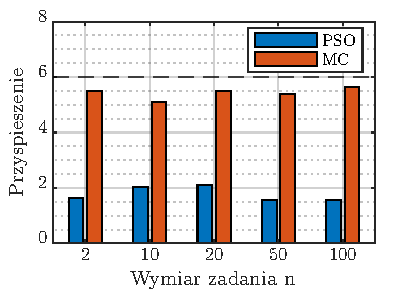
\includegraphics[width=0.9\textwidth]{grafiki/przyspieszenieMPI1.pdf}
\captionof{figure}{Przyspieszenie (6 rdzeni, 6 procesów, zad. 1.)}
\end{figure}

\end{column}
\begin{column}[t]{0.5\textwidth}

\begin{figure}[t]
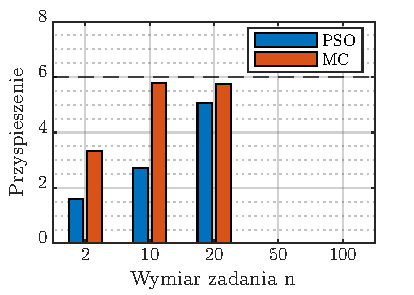
\includegraphics[width=0.9\textwidth]{grafiki/przyspieszenieMPI2.pdf}
\captionof{figure}{Przyspieszenie (6 rdzeni, 6 procesów, zad. 2.)}
\end{figure}

\end{column}
\end{columns}
\end{frame}



\subsection{OpenMP}
\begin{frame}{Implementacja PSO w OpenMP}
\begin{figure}[t]
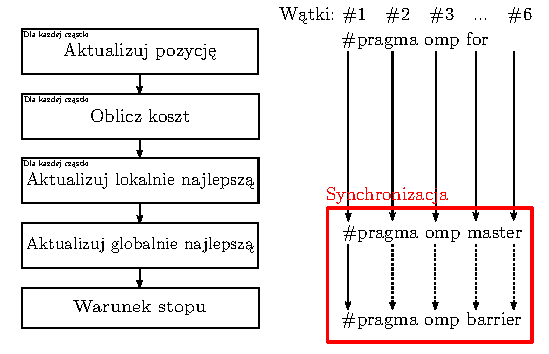
\includegraphics[width=0.9\textwidth]{grafiki/alg_OpenMP_synchronizacja.pdf}
\end{figure}
\end{frame}

\begin{frame}{Implementacja Monte Carlo w OpenMP}
\begin{figure}[t]
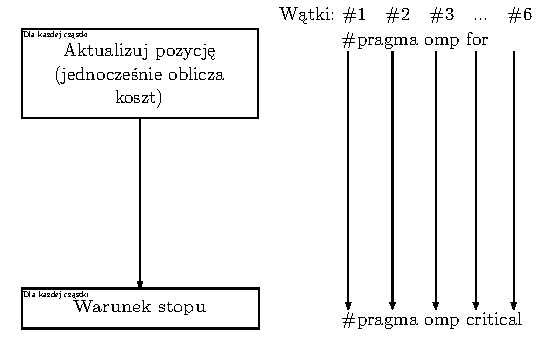
\includegraphics[width=0.9\textwidth]{grafiki/alg_OpenMP_MC.pdf}
\end{figure}
\end{frame}

\begin{frame}{Podsumowanie OpenMP}
\begin{itemize}
\item Brak synchronizacji w Monte Carlo skutkuje lepszymi przyspieszeniami.
\item Niezdefiniowany wynik paralelizacji pętli w funkcjach wywołanych z zrównoleglonej pętli w OpenMP.
\item Zarządzanie pamięcią może być trudne, np. generator PRNG.
\end{itemize}
\begin{columns}
\begin{column}[t]{0.5\textwidth}

\begin{figure}[t]
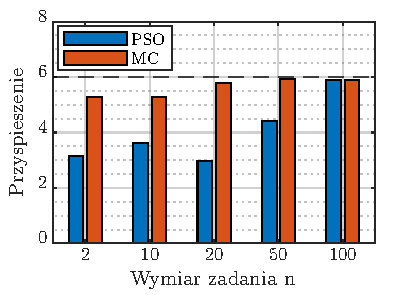
\includegraphics[width=0.9\textwidth]{grafiki/tabela_zad1_przyspieszenie.pdf}
\captionof{figure}{Przyspieszenie (6 rdzeni, 6 wątków, zad. 1.)}
\end{figure}

\end{column}
\begin{column}[t]{0.5\textwidth}

\begin{figure}[t]
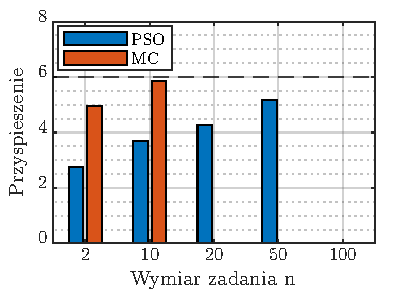
\includegraphics[width=0.9\textwidth]{grafiki/tabela_zad2_przyspieszenie.pdf}
\captionof{figure}{Przyspieszenie (6 rdzeni, 6 wątków, zad. 2.)}
\end{figure}

\end{column}
\end{columns}
\end{frame}


\subsection{CUDA}
\begin{frame}{Implementacja PSO w CUDA}
\begin{figure}[t]
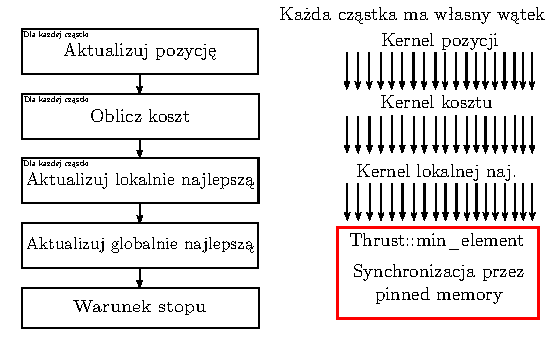
\includegraphics[width=0.9\textwidth]{grafiki/alg_CUDA_PSO.pdf}
\end{figure}
\end{frame}

\begin{frame}{Implementacja Monte Carlo w CUDA}
\begin{figure}[t]
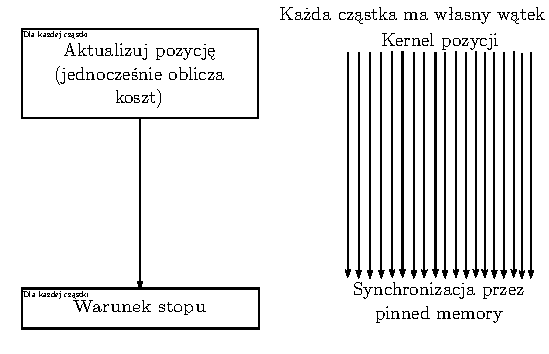
\includegraphics[width=0.9\textwidth]{grafiki/alg_CUDA_MC.pdf}
\end{figure}
\end{frame}

\begin{frame}{Podsumowanie CUDA}
\begin{itemize}
\item Porównywalne lub gorsze od implementacji CPU czasy obliczeń dla małej liczby cząsteczek.
\item Zadanie o $n \ = \ 200$ wymiarach z $1 \ 000 \ 000$ cząsteczek -- około $7 \ s$.
\item Zaprojektowanie optymalnej implementacji kodu to sztuka.
\begin{itemize}
\item Optymalne wykorzystanie mocy obliczeniowej przy 400 operacjach arytmetycznych \textit{float32} na jedną operację na pamięci.
\item Zaproponowana implementacja wykorzystuje $85\% $ przepustowości pamięci.
\item Subtelne zmiany mogą znacznie wpłynąć na czas obliczeń, np. \textit{blockSize}.
\end{itemize}
\end{itemize}
\begin{figure}[t]
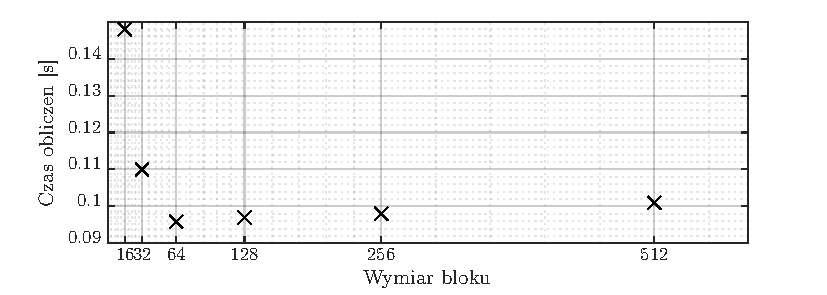
\includegraphics[width=0.8\textwidth]{grafiki/blocksizeplot.pdf}
\captionof{figure}{Czas obliczeń w zależności od \textit{blockSize}.}
\end{figure}
\end{frame}





\section{Wnioski}
\begin{frame}{Wnioski}
\begin{itemize}
\item W przypadku MPI przyspieszenie algorytmu PSO jest znacznie mniejsze niż przyspieszenie Monte Carlo -- w implementacji PSO dużo czasu poświęcane jest komunikacji międzyprocesowej - w każdej iteracji procesy muszą sprawdzić czy znana jest nowa globalna najlepsza wartość. Metoda Monte Carlo nie używa komunikacji w trakcie obliczeń - wiadomości wysyłane są jedynie po znalezieniu zadowalającego rozwiązania przez jeden z procesów.
\item Przy zastosowaniu metody MPI zmodyfikowany algorytm Monte Carlo z odpowiednio dobranymi parametrami (T o dużej wartości) prowadzi cząsteczkę do minimum lokalnego bez nadmiernego „skakania” po przestrzeni zadania jak widoczne jest to w niektórych przypadkach działania PSO.
\end{itemize}
\end{frame}

\begin{frame}{Wnioski cd.}
\begin{itemize}
\item OpenMP jest najbardziej efektywne biorąc pod uwagę ilość włożonej pracy, ale zarządzanie bardziej skomplikowanymi ścieżkami programu może być trudne.
\item CUDA daje najlepsze wyniki dla ogromnych liczb cząstek - optymalna implementacja jest trudna i bardzo pracochłonna.
\end{itemize}
\end{frame}

\end{document}